In this section we apply bandit algorithms on SA-problem and evaluate its performance on synthetic and real datasets. For synthetic example, we consider data transmission over a binary symmetric channel, and for real world examples, we use diabetes (PIMA indiana) and heart disease (Clevland) from UCI dataset. The experiments are set up as follows:

{\bf Synthetic:} We consider data transmission over two binary symmetric channels (BSCs). Channel $i=1,2$ flips input bit with probability $p_i$ where $p_1> p_2$. Transmission over channel $2$ costs $ c \in (0,1] $ units per bit. Input bits are generated with uniform probability. We set $p_1=.2$ and $p_2=.1$. For this example, $p_{12}=.26$ and $\delta_{12}=.8$. Thus, it satisfies weak dominance assumption for all $ 0<c <0 .1$ and $0 .26 \leq c < 1$.

We obtain a sensor acquisition setup from the datasets as follows: in each dataset, attributes related to physical observations are cheap and that obtained from medical tests are costly. Two svm classifiers (linear, $C=.01$) are trained for each dataset, one using only cheap attributes, and the other using all attributes. These classifiers then form sensors of a two stage SAP where classifier trained with cheap features is the first stage. Cost $c$ is defined as total cost of all attributes and total cost of cheap attributes multiplied by a scaling factor $\lambda$ (trade-off parmaeter for accuracy and costs). Specific details for each dataset is given below and the various error probabilities are listed in Table (\ref{tab:ErrorTable}).    

{\bf PIMA indians diabetes} dataset consists of $768$ instances and has $8$ attributes. The labels identify if the instances are diabetic or not. $6$ of the attributes (age, sex, triceps, etc.) obtained from physical observations, are cheap, and $2$ attributes (glucose and insulin) require expensive tests. First sensor of SAP is trained with $6$ cheap attributes and costs \$$6$. Total cost for all attributes is \$$30$. We set $c= 24\lambda$.

{\bf Heart disease} dataset consists of $297$ instance (without missing values) and has $13$ attributes. $5$ class labels $(0,1,2,3,4)$ are mapped to binary values by taking value $0$ as `absence' of disease and values $(1,2,3,4)$ as `presence' of disease. First senor of SAP is trained with $7$ attributes that costs  \$$1$ each. Total cost of all attributes is \$$568$. We set $c= 561\lambda$.


\centering
\begin{tabular}[c]{c|c|c|c|c } 
	\label{tab:ErrorTable}
	%			\caption{Possible binary tuples}
	
	dataset & $\gamma_1$ & $\gamma_2$ & $p_{12}$ & $\delta_{12}$\\ \hline 
	synthetic & .2 & .1 & .26 & .08\\  \hline
	diabetic & $0.3836 $ & $0.2808$ & $0.1986$ & 0.0778\\  \hline
	heart & $0.3051$ & $0.1695$ & $0.2373$ & 0.0732\\  \hline
\end{tabular}



\begin{figure}[!h]
	\centering
	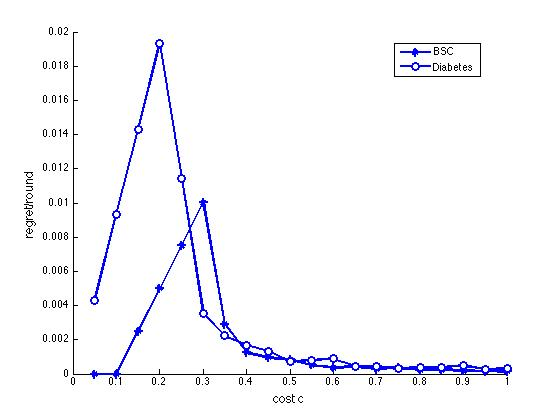
\includegraphics[scale=.4]{../Simulations/RegVsCost.jpg}
\end{figure}

\begin{figure}[!h]
	\centering
	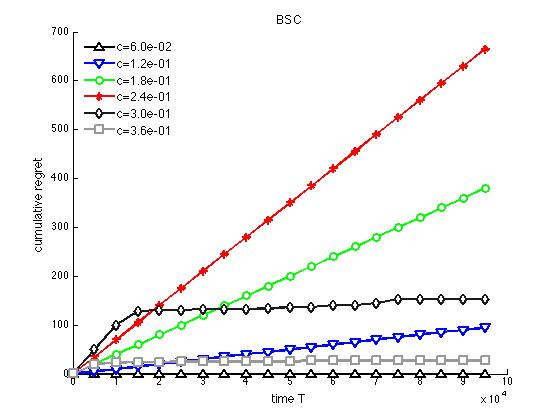
\includegraphics[scale=.4]{../Simulations/Synthetic/BSC.jpg}
\end{figure}
